\documentclass{article}
\usepackage{../fasy-hw}

%% UPDATE these variables:
\renewcommand{\hwnum}{3}
\title{Discrete Structures, Homework \hwnum}
\author{Braeden Hunt (Tinnittin)}
\collab{n/a}
\date{due: 5 March 2021}

\begin{document}

\maketitle

This homework assignment should be
submitted as a single PDF file both to D2L and to Gradescope.

General homework expectations:
\begin{itemize}
    \item Homework should be typeset using LaTex.
    \item Answers should be in complete sentences and proofread.
    \item You will not plagiarize.
    \item List collaborators at the start of each question using the \texttt{collab} command.
    \item Put your answers where the \texttt{todo} command currently is (and
        remove the \texttt{todo}, but not the word \texttt{Answer}).
\end{itemize}


% ============================================
% ============================================
\collab{n/a} \nextprob{Good Proofs}
% ============================================
% ============================================

Look through proofs in this textbook, or other books / papers.  Define five
qualities that you think are common among good proofs. Provide citations to
examples.


\paragraph{Answer}

\todo{your answer here}



% ============================================
% ============================================
\collab{\todo{}} \nextprob{Max of a Subset}
% ============================================
% ============================================

Let $(B,\leq)$ be a totally ordered finite set. Prove the following
statement: For all subsets $A \subseteq B$, the following inequality
holds: $\max(A) \leq \max(B)$.

\paragraph{Answer}

By definition of $A$, for all elements $x \in A, x\in B$. The definition of $\max(A)$ is that for all elements $x \in A, x \leq \max(A)$
This means that $\max(A) \in B$. So either $\max(A) = \max(B)$ by the definition of subsets or $ \max(A) < \max(B)$ by the definition of the $\max$ function.

It can also be shown that the negation cannot be true. Assume the negation: there exists a subset  $A \subseteq B$, the following inequality
holds: $\max(A) > \max(B)$. This means that there is an element, $x \in A$ that is greater than all elements in $B$. However, since $x \in A$,
 and $A \subseteq B$, $x \in B$ by the transitive property of elements in subsets. We are left with the result that $x>x$ which is a contradiction. 
 By assuming the negation, a contradiction arises.

% ============================================
% ============================================
\collab{\todo{}} \nextprob{Fibonacci}
% ============================================
% ============================================

The Fibonacci numbers are defined as follows:
$$
    F_i = \begin{cases}
            1 & i \in \{1,2\} \\
            F_{n-1}+F_{n-2} & \text{otherwise}
          \end{cases}
$$

Prove $\sum_{i=0}^n F_i = F_{n+2}-1$.

\paragraph{Answer}

\todo{your answer here}

% ============================================
% ============================================
\collab{\todo{}} \nextprob{US Coins}
% ============================================
% ============================================

Consider the four smallest denominations of US coins: $D=\{1,5,10,25\}$.  Prove, using
induction, that, for each $n \geq 1$, you can make $n$ cents using at most four
pennies.

\paragraph{Answer}
The claim we are trying to prove is that any $k = 0.01i$ where $i \in \{100, 101, 102...\}$ can be written in the form:

$k = 0.25q + 0.1d + 0.05n + 0.01p$ (or $i = 25q + 10d + 5n + p$ by substitution)
where $q$, $d$, $n$, and $p$ are all non-negative integers and $p<5$.

The base case is $i = 100$, which can be written as $i = 25(4) + 10(0) + 5(0) + 1(0) = 100$

The inductive assumption is that $j$ can expressed by $j = 25q + 10d + 5n + p$ such that $p<5$ and $j \geq 100$

Now consider $i=j+1$. We get the result $j+1 = 25q + 10d +5n + (p+1)$. This shows that we can write any value 
$i$ as that sum by adding one to $p$ for each increase in $i$.

In order to prove that the sum $i = 25q + 10d + 5n + p$ can be rewritten such that $p<5$, we will consider the Quotient Remainder Theorem.
We can see that any positive integer $a$ can be expresses as $a = bc + r$ where $0 \leq r \leq b$ and $b$ is a positive integer and $q$ is a non-negative integer.
Since $5n+p$ is a positive integer, we can replace them with $a=bc+r$ in $i$. We are left with  $i = 25q + 10d + bc+r$ where $b=5$ and $p=r$. 
The Quotient Remained Theorem states that $0 \leq r \leq b$. By substitution, we can see that $0 \leq p \leq 5$. This is what was to be shown.

\todo{your answer here}

% ============================================
% ============================================
\collab{n/a} \nextprob{Four Colors Suffice}
% ============================================
% ============================================

Read Chapters $4$ and $5$ of \emph{Four Colors Suffice}.

Use a ``minimal criminal'' argument to prove that if an edge is removed from a
tree, then the resulting graph has two connected components.

        \paragraph{Answer}

	A tree is defined as a connected graph that has no cycles. It follows that there is one and only one path from one vertex to any other vertex.
	
	The base case is the simplest tree, a graph $G$ with two vertices connected by one edge. By removing the edge, the resulting graph has two connected components. See Figure \ref{graph}.
	
	Assume that a tree $P$ is structured is such a way that it satisfies the condition if an edge is removed from $P$, then the resulting graph has 
	two connected components and that if a tree $G$ is created by adding an edge to $P$, it does not satisfy that condition. This makes the graph $G$ a
	minimal criminal. We can see that this forms a contradiction, however, as by adding an edge to $P$ to create $G$, we are creating a cycle. We are 
	connecting two existing vertices with an edge, creating a direct path between them, but as $P$ is a tree, there is already a path between those two vertices.
	This means that there are two paths between the vertices. Therefore, $G$ is not a tree. Thus, the minimal criminal cannot exist.
	Because there is no minimal criminal and there is a base case, the statement is true.

 \begin{figure}
\caption{Base Case}
\centering
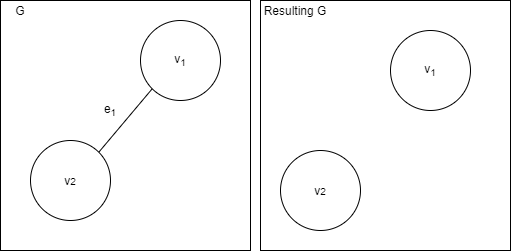
\includegraphics[width=0.5\textwidth]{images/graphBaseCase}
\label{graph}
\end{figure}

% ============================================
% ============================================
\collab{\todo{}}
\nextprob{Leonhard Euler}
% ============================================
% ============================================

Write a short (1-2 paragraph) biography of Leonhard Euler.
\textbf{In your own words}, describe who they are and why they are important in
the history of computer science.

If you use external resources, please provide
proper citations. If you do not use external sources, please write ``I did not
use any sources to write this biography'' as the last sentence of the
biography.

\paragraph{Answer}

\todo{your answer here}

% %% ... the bibliography
% \newpage
% \bibliographystyle{acm}
% \bibliography{biblio}

\end{document}

